%% UNIVERSIDADE FEDERAL DE MINAS GERAIS
%% Engenharia Aeroespacial
%% Trabalho de Conclusão de Curso
%% Autor: Laura Tameirao Sampaio Rodrigues
%% Matrícula: 2013025569
%% Data: 20/07/2018

%% Baseado em:
% ------------------------------------------------------------------------
% ------------------------------------------------------------------------
% abnTeX2: Modelo de Trabalho Academico (tese de doutorado, dissertacao de
% mestrado e trabalhos monograficos em geral) em conformidade com
% ABNT NBR 14724:2011: Informacao e documentacao - Trabalhos academicos -
% Apresentacao
% ------------------------------------------------------------------------
% ------------------------------------------------------------------------

\documentclass[
	% -- opções da classe memoir --
	12pt,				  % tamanho da fonte
	openright,		% capítulos começam em pág ímpar (insere página vazia caso preciso)
	twoside,			% para impressão em recto e verso. Oposto a oneside
	a4paper,			% tamanho do papel.
	% -- opções da classe abntex2 --
	%chapter=TITLE,		% títulos de capítulos convertidos em letras maiúsculas
	%section=TITLE,		% títulos de seções convertidos em letras maiúsculas
	%subsection=TITLE,	% títulos de subseções convertidos em letras maiúsculas
	%subsubsection=TITLE,% títulos de subsubseções convertidos em letras maiúsculas
	% -- opções do pacote babel --
	english,			% idioma adicional para hifenização
	french,				% idioma adicional para hifenização
	spanish,			% idioma adicional para hifenização
	brazil				% o último idioma é o principal do documento
	]{abntex2}

% ---
% Pacotes básicos
% ---
\usepackage{lmodern}			    % Usa a fonte Latin Modern
\usepackage[T1]{fontenc}		  % Selecao de codigos de fonte.
\usepackage{amsmath}
\usepackage[utf8]{inputenc}		% Codificacao do documento (conversão automática dos acentos)
\usepackage{lastpage}			    % Usado pela Ficha catalográfica
\usepackage{indentfirst}		  % Indenta o primeiro parágrafo de cada seção.
\usepackage{color}				    % Controle das cores
\usepackage{graphicx}			    % Inclusão de gráficos
\usepackage{microtype} 			  % para melhorias de justificação
% ---

% % ---
% % Pacotes adicionais, usados apenas no âmbito do Modelo Canônico do abnteX2
% % ---
% \usepackage{lipsum}				% para geração de dummy text
% % ---

% ---
% Pacotes de citações
% ---
\usepackage[brazilian,hyperpageref]{backref}	 % Paginas com as citações na bibl
\usepackage[alf]{abntex2cite}	% Citações padrão ABNT

% ---
% CONFIGURAÇÕES DE PACOTES
% ---

% ---
% Configurações do pacote backref
% Usado sem a opção hyperpageref de backref
\renewcommand{\backrefpagesname}{Citado na(s) página(s):~}
% Texto padrão antes do número das páginas
\renewcommand{\backref}{}
% Define os textos da citação
\renewcommand*{\backrefalt}[4]{
	\ifcase #1 %
		Nenhuma citação no texto.%
	\or
		Citado na página #2.%
	\else
		Citado #1 vezes nas páginas #2.%
	\fi}%
% ---

% ---
% Informações de dados para CAPA e FOLHA DE ROSTO
% ---
\titulo{Otimização estrutural de um painel reforçado utilizando os parâmetros de laminação}
\autor{Laura Tameirao Sampaio Rodrigues}
\local{Belo Horizonte, MG - Brasil}
\data{\today}
\orientador{Prof. Rodrigo de Sá Martins}
\coorientador{-}
\instituicao{%
  Universidade Federal de Minas Gerais -- UFMG
  \par
  Escola de Engenharia
  \par
  Engenharia Aeroespacial}
\tipotrabalho{Trabalho de Conclusão de Curso}
% O preambulo deve conter o tipo do trabalho, o objetivo,
% o nome da instituição e a área de concentração
\preambulo{Trabalho de conclusão de curso de Engenharia Aeroespacial na Universidade Federal de Minas Gerais, centrado na otimização de uma estrutura em material composto utilizando os parâmetros de laminação}
% ---


% ---
% Configurações de aparência do PDF final

% alterando o aspecto da cor azul
\definecolor{blue}{RGB}{41,5,195}

% informações do PDF
\makeatletter
\hypersetup{
     	%pagebackref=true,
		pdftitle={\@title},
		pdfauthor={\@author},
    	pdfsubject={\imprimirpreambulo},
	    pdfcreator={LaTeX with abnTeX2},
		pdfkeywords={abnt}{latex}{abntex}{abntex2}{trabalho acadêmico},
		colorlinks=true,       		% false: boxed links; true: colored links
    	linkcolor=blue,          	% color of internal links
    	citecolor=blue,        		% color of links to bibliography
    	filecolor=magenta,      		% color of file links
		urlcolor=blue,
		bookmarksdepth=4
}
\makeatother
% ---

% ---
% Espaçamentos entre linhas e parágrafos
% ---

% O tamanho do parágrafo é dado por:
\setlength{\parindent}{1.3cm}

% Controle do espaçamento entre um parágrafo e outro:
\setlength{\parskip}{0.2cm}  % tente também \onelineskip

% ---
% compila o indice
% ---
\makeindex
% ---

% ----
% Início do documento
% ----
\begin{document}

% Seleciona o idioma do documento (conforme pacotes do babel)
%\selectlanguage{english}
\selectlanguage{brazil}

% Retira espaço extra obsoleto entre as frases.
\frenchspacing

% ----------------------------------------------------------
% ELEMENTOS PRÉ-TEXTUAIS
% ----------------------------------------------------------
% \pretextual

% ---
% Capa
% ---
\imprimircapa
% ---

% ---
% Folha de rosto
% (o * indica que haverá a ficha bibliográfica)
% ---
\imprimirfolhaderosto*
% ---

% ---
% Inserir a ficha bibliografica
% ---

% Isto é um exemplo de Ficha Catalográfica, ou ``Dados internacionais de
% catalogação-na-publicação''. Você pode utilizar este modelo como referência.
% Porém, provavelmente a biblioteca da sua universidade lhe fornecerá um PDF
% com a ficha catalográfica definitiva após a defesa do trabalho. Quando estiver
% com o documento, salve-o como PDF no diretório do seu projeto e substitua todo
% o conteúdo de implementação deste arquivo pelo comando abaixo:
%
% \begin{fichacatalografica}
%     \includepdf{fig_ficha_catalografica.pdf}
% \end{fichacatalografica}

\begin{fichacatalografica}
	\sffamily
	\vspace*{\fill}					% Posição vertical
	\begin{center}					% Minipage Centralizado
	\fbox{\begin{minipage}[c][8cm]{13.5cm}		% Largura
	\small
	\imprimirautor
	%Sobrenome, Nome do autor

	\hspace{0.5cm} \imprimirtitulo  / \imprimirautor. --
	\imprimirlocal, \imprimirdata-

	\hspace{0.5cm} \pageref{LastPage} p. : il. (algumas color.) ; 30 cm.\\

	\hspace{0.5cm} \imprimirorientadorRotulo~\imprimirorientador

	\hspace{0.5cm} \imprimircoorientadorRotulo~\imprimircoorientador\\

	\hspace{0.5cm}
	\parbox[t]{0.9\textwidth}{\imprimirtipotrabalho~--~\imprimirinstituicao,
	\imprimirdata.}\\

	\hspace{0.5cm}
		1. Otimização.
		2. Materiais compostos.
		2. Parâmetros de laminação.
		I. \imprimirorientador.
		II. Universidade Federal de Minas Gerais.
		III. Escola de Engenharia.
		IV. \imprimirtitulo
	\end{minipage}}
	\end{center}
\end{fichacatalografica}
% ---

% % ---
% % Inserir errata
% % ---
% \begin{errata}
% Elemento opcional da \citeonline[4.2.1.2]{NBR14724:2011}. Exemplo:
%
% \vspace{\onelineskip}
%
% FERRIGNO, C. R. A. \textbf{Tratamento de neoplasias ósseas apendiculares com
% reimplantação de enxerto ósseo autólogo autoclavado associado ao plasma
% rico em plaquetas}: estudo crítico na cirurgia de preservação de membro em
% cães. 2011. 128 f. Tese (Livre-Docência) - Faculdade de Medicina Veterinária e
% Zootecnia, Universidade de São Paulo, São Paulo, 2011.
%
% \begin{table}[htb]
% \center
% \footnotesize
% \begin{tabular}{|p{1.4cm}|p{1cm}|p{3cm}|p{3cm}|}
%   \hline
%    \textbf{Folha} & \textbf{Linha}  & \textbf{Onde se lê}  & \textbf{Leia-se}  \\
%     \hline
%     1 & 10 & auto-conclavo & autoconclavo\\
%    \hline
% \end{tabular}
% \end{table}
%
% \end{errata}
% % ---

% ---
% Inserir folha de aprovação
% ---

% Isto é um exemplo de Folha de aprovação, elemento obrigatório da NBR
% 14724/2011 (seção 4.2.1.3). Você pode utilizar este modelo até a aprovação
% do trabalho. Após isso, substitua todo o conteúdo deste arquivo por uma
% imagem da página assinada pela banca com o comando abaixo:
%
% \includepdf{folhadeaprovacao_final.pdf}
%
\begin{folhadeaprovacao}

  \begin{center}
    {\ABNTEXchapterfont\large\imprimirautor}

    \vspace*{\fill}\vspace*{\fill}
    \begin{center}
      \ABNTEXchapterfont\bfseries\Large\imprimirtitulo
    \end{center}
    \vspace*{\fill}

    \hspace{.45\textwidth}
    \begin{minipage}{.5\textwidth}
        \imprimirpreambulo
    \end{minipage}%
    \vspace*{\fill}
   \end{center}

   Trabalho aprovado. \imprimirlocal, \today:

   \assinatura{\textbf{\imprimirorientador} \\ Orientador}
   \assinatura{\textbf{\imprimircoorientador} \\ Coorientador}
   \assinatura{\textbf{Nome} \\ Convidado 1}
   %\assinatura{\textbf{Professor} \\ Convidado 3}
   %\assinatura{\textbf{Professor} \\ Convidado 4}

   \begin{center}
    \vspace*{0.5cm}
    {\large\imprimirlocal}
    \par
    {\large\imprimirdata}
    \vspace*{1cm}
  \end{center}

\end{folhadeaprovacao}
% ---

% ---
% Dedicatória
% ---
\begin{dedicatoria}
   \vspace*{\fill}
   \centering
   \noindent
   \textit{Dedicatória: a fazer.} \vspace*{\fill}
\end{dedicatoria}
% ---

% ---
% Agradecimentos
% ---
\begin{agradecimentos}

Aos meus pais, Amilvana e Marcos, por me permitirem e me apoiarem a estudar todos esses anos na UFMG, e por todo o suporte que eles sempre me deram nas minhas escolhas profissionais.

Ao meu irmão, Victor, pela amizade e apoio durante todo este tempo.

Aos meus colegas de faculdade, especialmente, aos colegas de equipe do Aerodesign, por todo o companherismo.

Aos meus colegas e supervisores do estágio, com quem tive a oportunidade de grande aprendizado, por todo o apoio e ensino durante esses últimos meses.

Aos todos os meus professores pelo ensinamento passado durante os últimos anos.

Ao meu orientador, Prof. Helio de Assis, e ao Prof. Rodrigo Martins, pela ajuda e suporte na realização deste trabalho.

\end{agradecimentos}

% ---

% ---
% Epígrafe
% ---
\begin{epigrafe}
    \vspace*{\fill}
	\begin{flushright}
		\textit{
Epigrafe: a fazer.
%``I'm afraid that the following syllogism may be used by some in the future.
%\\~\\
%Turing believes machines think\\
%Turing lies with men\\
%Therefore machines do not think
%\\~\\
%Yours in distress,\\
%Alan''\\~\\
%(Alan Turing, Letter to Norman Routledge, 1952)
}
	\end{flushright}
\end{epigrafe}
% ---

% ---
% RESUMOS
% ---
% resumo em português
\setlength{\absparsep}{18pt} % ajusta o espaçamento dos parágrafos do resumo
\begin{resumo}
 % Segundo a \citeonline[3.1-3.2]{NBR6028:2003}, o resumo deve ressaltar o
 % objetivo, o método, os resultados e as conclusões do documento. A ordem e a extensão
 % destes itens dependem do tipo de resumo (informativo ou indicativo) e do
 % tratamento que cada item recebe no documento original. O resumo deve ser
 % precedido da referência do documento, com exceção do resumo inserido no
 % próprio documento. (\ldots) As palavras-chave devem figurar logo abaixo do
 % resumo, antecedidas da expressão Palavras-chave:, separadas entre si por
 % ponto e finalizadas também por ponto.

 A primeira versão deste Trabalho de Concusão de Curso consiste em uma revisão bibliográfica a respeito do tema: Otimização estrutural de um painel reforçado utilizando os parâmetros de laminação. As próximas versões irão conter mais detalhes da metodologia adotada e os resultados obtidos durante o desenvolvimento do trabalho.


 \textbf{Palavras-chave}: engenharia aeroespacial. otimização. materiais compostos. parâmetros de laminação. painel reforçado. nastran sol 200.
\end{resumo}

% % resumo em inglês
% \begin{resumo}[Abstract]
%  \begin{otherlanguage*}{english}
%    - to do -
%
%    \vspace{\onelineskip}
%
%    \noindent
%    \textbf{Keywords}: aerospace. missile. simulation. hardware-in-the-loop.
%    model based design. model based system engineering. test driven development.
%  \end{otherlanguage*}
% \end{resumo}
%
% % resumo em francês
% \begin{resumo}[Résumé]
%  \begin{otherlanguage*}{french}
%     - à faire -
%
%    \textbf{Mots-clés}: aérospatiale. missile. simulation. hardware-in-the-loop.
%    model based design. model based system engineering. test driven development.
%  \end{otherlanguage*}
% \end{resumo}
%
% % resumo em espanhol
% \begin{resumo}[Resumen]
%  \begin{otherlanguage*}{spanish}
%    - a hacer -
%
%    \textbf{Palabras clave}: aeroespacial. misil. simulación.
%    hardware-in-the-loop. model based design. model based system engineering.
%    test driven development.
%  \end{otherlanguage*}
% \end{resumo}

% ---

% % ---
% % inserir lista de ilustrações
% % ---
% \pdfbookmark[0]{\listfigurename}{lof}
% \listoffigures*
% \cleardoublepage
% % ---
%
% % ---
% % inserir lista de tabelas
% % ---
% \pdfbookmark[0]{\listtablename}{lot}
% \listoftables*
% \cleardoublepage
% % ---

% ---
% inserir lista de abreviaturas e siglas
% ---

\begin{siglas}

  \item[PL] \emph{Parâmetros de laminação}
  \item[CLT] \emph{Classical Theory of Lamination}
  \item[FEM] \emph{Finite Element Model}


\end{siglas}

% ---
%
% % ---
% % inserir lista de símbolos
% % ---
% % 
% \begin{simbolos}
%   \item[$ \alpha $] teste-alfa
% \end{simbolos}

% % ---

% ---
% inserir o sumario
% ---
\pdfbookmark[0]{\contentsname}{toc}
\tableofcontents*
\cleardoublepage
% ---



% ----------------------------------------------------------
% ELEMENTOS TEXTUAIS
% ----------------------------------------------------------
\textual

% ----------------------------------------------------------
% Objetivos
% ----------------------------------------------------------
\chapter{Objetivos}

Como trabalho final do curso de graduação em Engenharia Aeroespacial na Universidade Federal de Minas Gerais, este trabalho de pesquisa foi realizado no âmbito de uma otimização estrutural de um painel reforçado utilizando como variáveis de otimização os parâmetros de laminação de cada componente estrutural.
Visando otimizar a estrutura de um painel reforçado quando submetido à uma determinada carga de compressão, será feito um modelo em elementos finitos utilizando o \emph{software FEMAP}. O revetimento do painel e os reforçadores serão otimizada utilizando a SOL 200 do \emph{Nastran} e análises de flambagem, SOL 105, serão realizadas visando obter os modos de flambagem da estrutura.

O objetivo inicial da otimização é obter as propriedades de um laminado que suporte a maior carga de flambagem, mantendo as espessuras do revestimento e a geometria e espessuras dos reforçadores constantes, portanto, variando somente as propriedades do laminado. Os parâmentros de laminação serão utilizados como variáveis de projeto e serão os resultados obtidos da otimização.

O outro objetivo do trabalho é criar um banco de dados para um determinado valor de espessura do laminado. Com este banco de dados de laminados será possível obter a sequência e os ângulos de cada lâmina do laminado com base nos valores de propriedades do laminado que foram otimizados.


% ----------------------------------------------------------
% Justificativa
% ----------------------------------------------------------
%\chapter{Justificativa}

A computação vem tomando um espaço cada vez maior nos processos industriais.
Tarefas antes dadas apenas a humanos podem ser realizadas atualmente por programas especializados de forma muito mais rápida e eficiente.
Na engenharia, cada vez mais etapas da concepção de um produto (desde a definição de parâmetros iniciais até sua fabricação em massa) são realizadas por computadores.

Ainda assim, o desenvolvimento de \emph{softwares} permanece uma tarefa complicada e direcionada apenas a especialistas.
Ademais, programas mais complexos muitas vezes não são inteligíveis exceto para seu criador.
Tais fenômenos dificultam o uso da ferramenta computacional, que poderia facilitar muito o andamento dos processos, mas em vez disso cria empecilhos que diminuem a produtividade.

É com base nessa problemática que metodologias bem definidas de projeto de \emph{software} podem ser úteis.
A Engenharia de Sistemas Baseada em Modelos (MBSE), por exemplo, fornece ferramentas de análise de programas que independem de implementações.
Isso significa que, ao trabalhar com os modelos propostos pela MBSE, os projetistas não têm de se preocupar com minúcias de código e erros técnicos, como dificuldades de compilação, incompatibilidades de sistemas operacionais, falta de drivers, dentre outros empecilhos que desviam a atenção da lógica do programa.
A partir dos modelos desenvolvidos, pode-se inclusive gerar código automaticamente para uma plataforma desejada.
Essa técnica pode, portanto, eximir do projetista conhecimentos mais aprofundados de programação.

O desenvolvimento dirigido pelos testes, por sua vez, promove uma validação mais abrangente do código.
Uma vez definida a metodologia para aplicação dos testes, os códigos podem ser direcionados mais diretamente para o cumprimento de requisitos.
A análise dos códigos é, então, facilitada, o que ajuda a garantir sua robustez e evitar falhas.
No setor aeroespacial, falhas custam bastante dinheiro e, por vezes, vidas.
A situação é mais crítica ainda quando se trata do setor de defesa, o que justifica o grande interesse em códigos robustos.


% ----------------------------------------------------------
% Introdução (exemplo de capítulo sem numeração, mas presente no Sumário)
% ----------------------------------------------------------
\chapter[Introdução]{Introdução}

A utilização de materiais compostos em estruturas primárias tem aumentado gradualmente nas últimas décadas. Atualmente, no setor aeronáutico, estruturas primárias como asas, fuselagens e empenagens possuem a tendência de serem projetadas utilizando painéis reforçados constituídos de material composto. Isto se deve ao fato de as estruturas em materiais compostos possuírem elevadas resistência e rigidez em relação a densidade \cite{herencia2007optimization}. Além disso, variando-se a sequência do laminado e os ângulos de laminação, as propriedades do material composto podem ser otimizadas em vista do componente estrutural no qual o laminado será aplicado, apresentando um potencial de uso bastante elevado.

No decorrer dos anos, diversas técnicas de otimização foram desenvolvidas para auxiliar nos processos de obtenção do laminado ótimo para cada uso. Algumas das técnicas de otimização dos materiais compostos envolvem a variação do número de camadas do laminado e dos ângulos de laminação, e assumem que o material possui propriedades ortotrópicas, conforme utilizado por \cite{schmit1973optimum}. No entanto, segundo \cite{chamis1969buckling} pelo fato de os materiais compostos poderem apresentar características anisotrópicas, resultados não conservativos podem ser obtidos, durante otimizações nas quais o comportamento em flambagem é observado, caso a anisotropia em flexão dos materiais não seja considerada. A otimização do número de camadas e dos ângulos de laminação de cada camada demanda um elevado custo computacional e consiste em um processo de otimização não linear com variáveis discretas e que possui um espaço de projeto não convexo.

Visando solucionar o problema de otimização das variáveis discretas da sequência de laminação dos materiais compostos, \cite{miki1991optimum} propôs a utilização dos parâmetros de laminação. O método proposto por \cite{miki1991optimum}, considera que a rigidez no plano e a rigidez flexural de materiais compostos que possuem laminados simétricos e ortotrópicos são funções dos parâmetros de laminação, e esses parâmetros dependem da sequência de laminação. Com isso, os parâmetros de laminação podem ser utilizados como as variáveis de projeto durante a otimização e os pontos ótimos de projeto podem ser obtidos em função desses parâmetros e da função objetivo.

O objetivo deste trabalho de conclusão de curso, é portanto, descrever um processo de otimização de um painel reforçado em material composto utilizando os parâmetros de laminação e as espessuras do revestimento e do reforçador como variáveis de projeto. O problema foi dividido em duas etapas, na qual a primeira consistiu em validar o otimizador utilizado. Para isso, comparou-se um modelo de um painel reforçado em material metálico com um painel reforçado proposto por \cite{niu1997airframe}. Após a validação do otimizador, fez-se a otimização do painel reforçado em material composto utilizando os parâmetros de laminação e aplicando restrições de projetos presentes na indústria aeronáutica. A função objetivo da otimização é obter uma estrutura mais leve e que suporte a carga de compressão aplicada, variando as propriedades do material e as espessuras do revestimento e do reforçador. Nesta etapa, assumiu-se que os laminados dos reforçadores e do revestimento eram simétricos e ortotrópicos.

%\section{Desenvolvimento histórico}

%\subsection{\emph{Model Driven Architecture}}

%\begin{enumerate}
%  \item \emph{Computational Independent Model} -- CIM:\\
%A primeira etapa do projeto se refere às especificações %do código, escritas em linguagem humana.
%\end{enumerate}


% ----------------------------------------------------------
\chapter[Materiais Compostos]{Materiais Compostos}

\section{Desenvolvimento histórico}
A implementação do uso de materiais compostos na indústria aeronáutica civil e militar seguiu os estágios típicos da implementação de qualquer nova tecnologia no mercado. Segundo \cite{kassapoglou2013design}, primeiramente o uso da tecnologia de materiais compostos foi limitado às estruturas secundárias visto que minimizavam os riscos envolvidos e também possibilitava a coleta de dados, o que viabilizava uma melhor compreensão do comportamento das estruturas que possuiam essa tecnologia.

De acordo com \cite{daniel2006engineering}, em 1942 o primeiro barco constiuído de fibra de vidro foi fabricado, e nos anos 1950 as primeiras aplicações com materiais compostos em mísseis foram realizadas. Referindo-se a indústria aeronáutica no último século, o primeiro uso de materiais compostos mais avançados, segundo \cite{kassapoglou2013design}, ocorreu no final da década de 1950 na aeronave \emph{Akaflieg Phonix FS-24}. Essa aeronave consistiu em um planador projetado por professores e alunos da Universidade de Stuttgart e foi construído, inicialmente de madeira balsa, e posteriormente teve sua estrutura alterada para um sanduíche de compósitos de fibra de vidro com madeira tipo balsa. Após isso, no fim dos anos 1960, com a nova geração de materiais compostos avançados, como o carbono, a indústria de helicópteros foi a primeira a utilizá-los em estruturas primárias, destacando o projeto do \emph{Aerospatiale AS-341 Gazelle}. Este helicóptero foi considerado um dos mais modernos na época, não só porque ele possuía um inovador rotor de cauda reduzindo drasticamente a emissão de ruídos, mas também, pelo fato de as pás do rotor principal serem constituídas de material composto.

Por volta dos anos 1970 as primeiras aeronaves majoritariamente constituídas de materiais compostos começaram a surgir. Essas aeronaves eram pequenas e normalmente para uso recreativo ou para acrobacias, visto que com o uso de materiais compostos era possível obter uma redução de peso estrutural e portanto, aeronaves mais rápidas e ágeis quando comparadas às aeronaves da época. O uso de material composto teve início em aeronaves pequenas também pelo fato de os requisitos de certificação estrutural para aeronaves menores serem mais facilmente cumpridos quando comparados aod requisitos das aeronaves de grande porte. Além disso, de acordo com \cite{kassapoglou2013design}, a performance dos materias compostos não era completamente conhecida, por exemplo, a sensitividade desse tipo de material ao dano por impacto e suas implicações para o projeto só foram ser melhor conhecidas no final dos anos 1970. Portanto, somente no final dos anos 1970 e início dos anos 1980 que a utilização de materiais compostos começou a ser expandida para aeronaves de porte maior, como a concepção da empenagem horizontal do \emph{Boeing 737}, que era uma estrutura primária construída de um sanduíche de materias compostos. Seguindo a aplicação em grande escala de materiais compostos, destaca-se o \emph{Airbus A320}, no qual tanto a empenagem horizontal e a vertical, quanto as superfícies de controle foram projetadas e fabricadas utilizando material composto.

A proxíma aplicação significante desse tipo de material em estruturas primárias foi no início dos anos 1990 com o \emph{Boeing 777}, em que além das empenagens e superfícies de controle, as vigas principais do piso eram constituídas de material composto.
Segundo \cite{daniel2006engineering}, o maior sinal de aceitação do uso de materiais compostos na indústria aeronáutica civil, ocorreu no \emph{Boeing 787 Dreamliner}, em que materiais como carbono/\emph{epoxy} e grafite/titânio constituíam cerca de 50\% do peso da aeronave, incluindo majoritariamente asas e fuselagem. Destaca-se também o \emph{Airbus A380}, que utiliza materiais compostos, incluindo o \emph{GLARE}, um laminado híbrido de fibra de vidro/\emph{epoxy}/alumínio, que combina as vantagens e desvantagens dos materiais metálicos e compostos.

Observa-se, portanto, que o uso dos materiais compostos vem aumentando de maneira significativa na indústria aeronáutica. Uma maneira de perceber o aumento do uso de materiais compostos nessa indústria é com base na \autoref{fig_usecomposites}, em que fica claro o aumento percentual da utilização desse tipo de material em relação ao peso das estruturas de vários modelos de aeronaves.

\begin{figure}[h]
	\caption{\label{fig_usecomposites}Uso de materiais compostos na indústria aeronáutica}
  \centering
  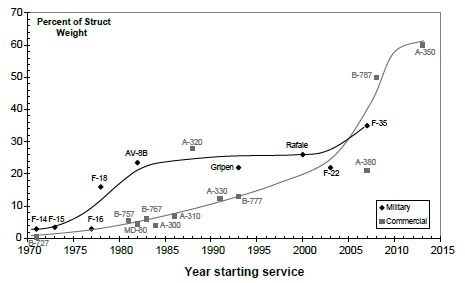
\includegraphics[scale=1.1]{figura/UseOfComposites}
	\legend{Fonte: \cite[p. 6]{kassapoglou2013design}}
\end{figure}

\section{Visão geral}
De acordo com \cite{daniel2006engineering}, os materiais compostos possuem diversas vantagens de utilização em relação aos materiais metálicos como a elevada resistência, a elevada rigidez, a vida longa em fadiga, a baixa densidade e a alta adaptabilidade em relação a função de utilização pretendida pela estrutura. A superior perfomance estrutural dos materiais compostos se deve basicamente às elevadas resistência e rigidez específicas e à anisotropia do material, visto que devido à esta última característica, o material composto possui diversos graus de liberdade para uma configuração ótima do laminado. No geral, devido ao elevado número de graus de liberdade é possível realizar a otimização do laminado em material composto para diversas restrições de projeto e objetivos, como menor peso estrutural, máxima estabilidade dinâminca e/ou menor custo de fabricação. No entanto, todo o processo requer um confiável banco de dados das propriedades dos materiais, métodos de análises estruturais, técnicas de modelagem e simulações padronizadas e certificadas. Logo, devido às numerosas opções disponíveis, os processos e análises acabam se tornando mais complexos e custos em relação aos dos materiais convencionais.

Os materiais compostos possuem algumas limitações de uso em relação ao materiais metálicos. Do ponto de vista da micromecânica, as fibras dos materiais compostos possuem uma grande variabilidade nas propriedades de resistência e concentradores de tensão locais reduzem consideravelmente a resistência a tração das estruturas projetadas em materiais compostos. Em relação a macromecânica, a anisotropia do material pode ser utilizada considerada como uma vantagem visto que o comportamento do material pode ser variado, no entando, esta mesma característica faz com que as análises desses materiais sejam muito mais complexas \cite{daniel2006engineering}.

\section{Teoria Clássica da Laminação}
De acordo com \cite{daniel2006engineering} para o desenvolvimento da Teoria Clássica da Laminação, assumem-se as seguintes premissas e restrições:
\begin{enumerate}
  \item Cada lâmina do laminado é quasi-homogênea e ortotrópica;
	\item O laminado é fino com as suas dimensões laterais muito maiores do que a sua espessura e é carregado somente no plano, isto é, o lamninado e suas lâminas (exceto as bordas) estão em um estado plano de tensão ($\sigma_z = \tau_{xz} = \tau_{yz} =  $ 0);
	\item Todos os deslocamentos são pequenos comparados com a espessura do laminado ($|u|,|v|,|w| \ll h$);
	\item Deslocamentos são contínuos ao longo da espessura;
	\item Deslocamentos no plano variam linearmente ao longo da espessura do laminado, isto é, os deslocamentos $\emph u$ e $\emph v$ nas direções $\emph x$ e $\emph y$ são funções lineares de $\emph z$;
	\item Linhas retas normais à superfície média permanece reta e normal à essa superfície após a deformação. Isto implica que as deformações transversais de cisalhamento $\gamma_{xz}$ e $\gamma_{yz}$ são nulas;
	\item As relações deformações-deslocamentos e tensões-deformações são lineares;
	\item Distâncias normais à superfície média permanecem constantes, isto é, o deslocamento transversal normal, $\varepsilon_{z}$ é zero. Isto implica que o deslocamento transversal $\emph w$ é independente da coordenada de espessura $\emph z$.
\end{enumerate}

\subsection{Relações entre deformações e deslocamentos}
Seguindo a \autoref{fig_laminatedeformation} como referência, tem-se que o plano $\emph x-y$ é o plano médio do laminado, ou seja, é equidistante do laminado mais superior e do mais inferior. Portanto, este plano é chamado de \emph{Plano médio} ou \emph{Plano de referência}.

\begin{figure}[h]
	\caption{\label{fig_laminatedeformation}Seção do laminado antes (ABCD) e depois da deformação (A'B'C'D')}
  \centering
  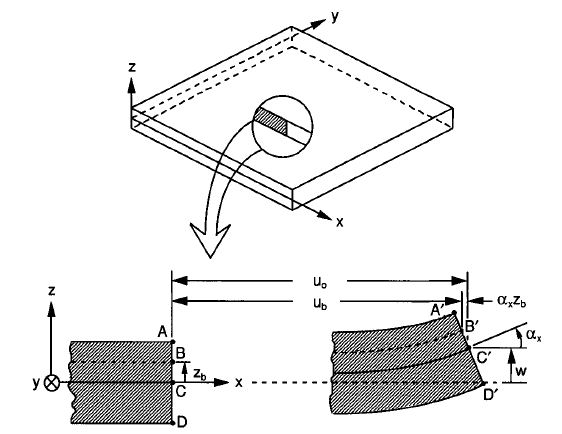
\includegraphics[scale=1.0]{figura/LaminateDeformation}
	\legend{Fonte: \cite{daniel2006engineering}}
\end{figure}

Tem-se que os deslocamentos no plano $u_0$ e $v_0$ nas direções $\emph x$ e $\emph y$ e o deslocamento fora do plano $w$ na direção $\emph z$ são funções somente de x e y, como mostrado a seguir.
\begin{equation} \label{displacements}
\begin{split}
u_{0}=u_{0}(x,y)\\
v_{0}=v_{0}(x,y)\\
w=f(x,y)
\end{split}
\end{equation}
E que as rotações ao longo dos eixos x e y são dadas por:
\begin{equation} \label{rotations}
\begin{split}
\alpha_{x}=\dfrac{\partial w} {\partial x}\\
\alpha_{y}=\dfrac{\partial w} {\partial y}
\end{split}
\end{equation}

Portanto, os componentes de deslocamentos de um ponto $B$ de coordenada $z_b$, onde z é a coordenada na espessura do laminado, são:
\begin{equation} \label{displacements_B}
\begin{split}
u=u_{0} - \dfrac{\partial w}{\partial x}\\
v=v_{0} - \dfrac{\partial w}{\partial y}
\end{split}
\end{equation}

Para pequenos deslocamentos, as relações clássicas de deformação e deslocamento no campo elástico são dadas por:
\begin{equation} \label{Strain_Displacement}
\begin{gathered}
\varepsilon_{x} = \dfrac{\partial u}{\partial x} = \dfrac{\partial u_0}{\partial x} - z\dfrac{\partial^2 w}{\partial x^2}\\~\\
\varepsilon_{y} = \dfrac{\partial v}{\partial y} = \dfrac{\partial v_0}{\partial y} - z\dfrac{\partial^2 w}{\partial y^2}\\~\\
\gamma_{xy} = \gamma_z = \dfrac{\partial u}{\partial y} + \dfrac{\partial v}{\partial x} = \dfrac{\partial u_0}{\partial y} + \dfrac{\partial v_0}{\partial x} - 2z\dfrac{\partial^2 w}{\partial x\partial y}
\end{gathered}
\end{equation}

Sabe-se ainda, por definição, que:
\begin{equation} \label{Strain_Curvatures}
\begin{gathered}
\varepsilon^0_{x} = \dfrac{\partial u_o}{\partial x}\\~\\
\varepsilon^0_{y} = \dfrac{\partial v_o}{\partial y}\\~\\
\gamma^0_{xy} = \gamma^0_z= \dfrac{\partial u_0}{\partial y} + \dfrac{\partial v_0}{\partial x}\\~\\
\kappa_x = -\dfrac{\partial^2 w}{\partial x^2}\\~\\
\kappa_y = -\dfrac{\partial^2 w}{\partial y^2}\\~\\
\kappa_{xy} = \kappa_z = -2\dfrac{\partial^2 w}{\partial x\partial y}
\end{gathered}
\end{equation}

Portanto, as deformações em qualquer ponto do laminado podem ser relacionadas às deformações do plano e às curvaturas do laminado como mostrado a seguir:

\begin{equation} \label{matrix_strain}
\begin{bmatrix}
    \varepsilon_{x} \\
    \varepsilon_{y} \\
    \gamma_{z} \\
\end{bmatrix}
=
\begin{bmatrix}
		\varepsilon^0_{x} \\
		\varepsilon^0_{y} \\
		\gamma^0_{z} \\
\end{bmatrix}
+z
\begin{bmatrix}
    \kappa_{x} \\
    \kappa_{y} \\
    \kappa_{z} \\
\end{bmatrix}
\end{equation}

\subsection{Relações entre tensões e deformações de uma lâmina dentro de um laminado}
Considera uma lâmina específica, \emph{k} em um laminado multidirecional, na qual a distância \emph{$z_k$} se refere a distância da lâmina ao plano de referência do Laminado. Tem-se que as relações de tensão-deformação para essa lâmina, no sistema de coordenada do laminado valem:

\begin{equation} \label{matrix_stress_strain}
\begin{bmatrix}
    \sigma_{x} \\
    \sigma_{y} \\
    \tau_{s} \\
\end{bmatrix}_k
=
\begin{bmatrix}
		Q_{xx} & Q_{xy} & Q_{xs} \\
		Q_{yx} & Q_{yy} & Q_{ys} \\
		Q_{sx} & Q_{sy} & Q_{ss} \\
\end{bmatrix}_k
\begin{bmatrix}
    \varepsilon_{x} \\
    \varepsilon_{y} \\
    \gamma_{s} \\
\end{bmatrix}_k
\end{equation}

Substituindo a \autoref{matrix_strain} na \autoref{matrix_stress_strain} tem-se, de forma generalizada, a seguinte expressão para as deformações:

\begin{equation} \label{general_stress_strain}
		[\sigma]^k_{x,y}=[Q]^k_{x,y}[\varepsilon^0]_{x,y}+z[Q]^k_{x,y}[\kappa]_{x,y}
\end{equation}

Nota-se, portanto, das \autoref{matrix_strain} e \autoref{general_stress_strain} que mesmo que as deformações variem linearmente, não necessariamente as tensões variam da mesma maneira. Devido à discontinuidade da matriz de rigidez $[Q]_{x,y}$ ao longo das lâminas do laminado, as tensões também podem variar de forma discontínua ao longo das lâminas.

\subsection{Relações envolvendo forças e momentos resultantes}
Tendo como referência a \autoref{fig_laminateforces} e sabendo que as tensões ao longo do laminado variam devido às diferentes matrizes de rigidez de cada lâmina específica, pode-se fazer uma integração para obter forças e momentos resultantes.

\begin{figure}[h]
	\caption{\label{fig_laminateforces}Elemento de uma lâmina com forças e momentos resultantes}
  \centering
  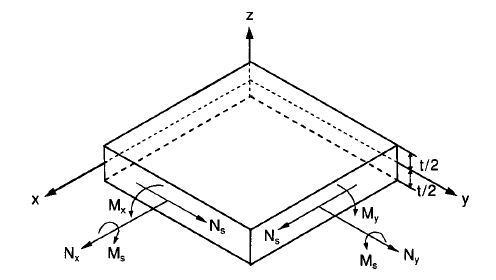
\includegraphics[scale=1.0]{figura/LaminateForcesMoments}
	\legend{Fonte: \cite{daniel2006engineering}}
\end{figure}

As expressões seguintes se relacionam a essas forças e momentos resultantes.

\begin{equation} \label{ForcesMoments}
\begin{gathered}
N^k_{x}=\int^{t/2}_{-t/2}\sigma_x\emph{dz}\\~\\
N^k_{y}=\int^{t/2}_{-t/2}\sigma_y\emph{dz}\\~\\
N^k_{s}=\int^{t/2}_{-t/2}\tau_s\emph{dz}\\~\\
M^k_{x}=\int^{t/2}_{-t/2}\sigma_x z\emph{dz}\\~\\
M^k_{y}=\int^{t/2}_{-t/2}\sigma_y z\emph{dz}\\~\\
M^k_{s}=\int^{t/2}_{-t/2}\tau_s z\emph{dz}
\end{gathered}
\end{equation}

Em que $\emph{z}$ é a coordenada da lâmina na seção do laminado, $\emph{t}$ é a espessura da lâmina, $N^k_i$ são as forças ($\emph{x, y, s}$) por unidade de comprimento e $M^k_i$ são os momentos ($\emph{x, y, s}$) por unidade de comprimento. E no caso de um laminado com diversas lâminas, a força e o momento total são obtidos fazendo o somatório dos efeitos de cada lâmina. Tem-se, portanto, as seguintes expressões:

\begin{equation} \label{SumForcesMoments}
\begin{gathered}
\begin{bmatrix}
    N_{x} \\
    N_{y} \\
    N_{s} \\
\end{bmatrix}_k
= \sum^n_{k=1} \int^{z_k}_{z_{k-1}}
\begin{bmatrix}
    \sigma_{x} \\
    \sigma_{y} \\
    \tau_{s} \\
\end{bmatrix}_k
\emph{dz} \\~\\
\begin{bmatrix}
    M_{x} \\
    M_{y} \\
    M_{s} \\
\end{bmatrix}_k
= \sum^n_{k=1} \int^{z_k}_{z_{k-1}}
\begin{bmatrix}
    \sigma_{x} \\
    \sigma_{y} \\
    \tau_{s} \\
\end{bmatrix}_k
z\emph{dz}
\end{gathered}
\end{equation}

Substituindo a \autoref{matrix_stress_strain} na \autoref{SumForcesMoments}, tem-se:
\begin{equation} \label{SumForcesMoments_general}
\begin{gathered}
N_{x,y} =
\begin{matrix}
[\sum^n_{k=1}[Q]^k_{x,y}({z_k} -{z_{k-1}})]
\end{matrix}
[\varepsilon^0]_{x,y} +
\begin{matrix}
[\sum^n_{k=1}[Q]^k_{x,y}({z^2_k} -{z^2_{k-1}})]
\end{matrix}
[\kappa]_{x,y}\\~\\
M_{x,y} =
\begin{matrix}
[\frac{1}{2}\sum^n_{k=1}[Q]^k_{x,y}({z^2_k} -{z^2_{k-1}})]
\end{matrix}
[\varepsilon^0]_{x,y} +
\begin{matrix}
[\frac{1}{3}\sum^n_{k=1}[Q]^k_{x,y}({z^3_k} -{z^3_{k-1}})]
\end{matrix}
[\kappa]_{x,y}
\end{gathered}
\end{equation}

Por definição tem-se as três matriz de rigidez do laminado como:
\begin{equation} \label{ABD_definition}
\begin{gathered}
A_{ij} = \sum^n_{k=1}[Q]^k_{ij}({z_k} -{z_{k-1}})\\~\\
B_{ij} =\frac{1}{2}\sum^n_{k=1}[Q]^k_{ij}({z^2_k} -{z^2_{k-1}})\\~\\
D_{ij} = \frac{1}{3}\sum^n_{k=1}[Q]^k_{ij}({z^3_k} -{z^3_{k-1}})
\end{gathered}
\end{equation}

Portanto, em geral, substituindo \autoref{ABD_definition} na \autoref{SumForcesMoments_general}, pode-se representar as forças e momentos resultantes em função das matrizes de rigidez [A], [B] e [D] como segue:
\begin{equation} \label{ABD_definition}
\begin{gathered}
\begin{bmatrix}
    N \\
    M \\
\end{bmatrix}
=
\begin{bmatrix}
		A & B \\
		B & D \\
\end{bmatrix}
\begin{bmatrix}
    \varepsilon^0 \\
    \kappa \\
\end{bmatrix}
\end{gathered}
\end{equation}

Para cada uma das matrizes de rigidez [A], [B] e [D] tem os seguintes significados físicos:
\begin{itemize}
\item Matriz [A]:
\item Matriz [B]:
\item Matriz [D]:
\end{itemize}

\section{Parâmetros de laminação}
\[
\begin{bmatrix}
    \xi_{11}^2       & x_{12} & x_{13} & \dots & x_{1n} \\
    x_{21}       & x_{22} & x_{23} & \dots & x_{2n} \\
    \hdotsfor{5} \\
    x_{d1}       & x_{d2} & x_{d3} & \dots & x_{dn}
\end{bmatrix}
=
\begin{bmatrix}
    x_{11} & x_{12} & x_{13} & \dots  & x_{1n} \\
    x_{21} & x_{22} & x_{23} & \dots  & x_{2n} \\
    \vdots & \vdots & \vdots & \ddots & \vdots \\
    x_{d1} & x_{d2} & x_{d3} & \dots  & x_{dn}
\end{bmatrix}
\]

\section{Práticas de projeto adotadas}
Esta seção apresenta regras e práticas relevantes utilizadas durante o projeto de estruturas em materiais compostos na indústria aeronáutica.

\subsection{Laminados simétricos}
Os laminados que possuem um sequência	de ângulos das lâminas simétrico em relação ao plano médio, são chamados de laminados simétricos. Conforme descrito por \cite{mil2002handbook} e \cite{niucomposite}, a maior vantagem da utilização de um laminado simétrico é o desacoplamento entre o comportamento de membrana e flexão da estrutura.

Em um laminado simétrico, conforme notação apresentada na \autoref{fig_laminate} e conforme a \autoref{eq_matrixB} matriz [B] do laminado se anula.

\begin{figure}[h]
	\caption{\label{fig_laminate}Notação para espessura do laminado e sequência das lâminas}
  \centering
  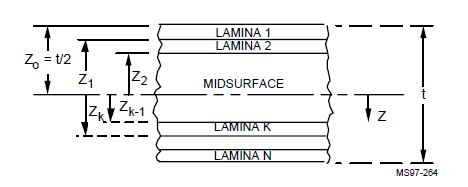
\includegraphics[scale=1.0]{figura/Laminate}
	\legend{Fonte: \cite{mil2002handbook}}
\end{figure}

\begin{equation} \label{eq_matrixB}
B_{ij}
=
\sum_{k=1}^N (\overline{Q}_{ij})_k [z_k^2 - (z_{k-1})^2]
\end{equation}

Sabe- se que $ \overline{Q}_{ij} $ corresponde a rigidez da lâmina. E sabe-se também que a matriz $ B_{ij} $ é a responsável pelo acomplamento entre a reposta no plano e a flexão do laminado. Portanto, conforme \cite{nasa1997guidelines}, quando a matriz $ B_{ij} $ não é zerada, um carregamento no plano induz curvaturas, e momentos de flexão induzem deformações no plano. Nota-se pela \autoref{eq_matrixB} que a matriz $ B_{ij} $ possui termos da coordenada z elevados ao quadrado, portanto, quando o laminado possui simetria geométrica e de materiais em relação ao plano médio, este termo é zerado.

\subsection{Laminados balanceados}
Os laminados balanceados são aqueles em que todas as lâminas, com exceção das de 0$^{\circ}$ e das de 90$^{\circ}$, devem ocorrer em pares de $ +\theta $ e $ -\theta $ acima e abaixo do plano médio do laminado. Para o conjunto de laminados compostos por lâminas com ângulos 0/$\pm$45/90, cada lâmina de +45$^{\circ}$ deve ser acompanhada de um lâmina de -45$^{\circ}$.
Laminados balanceados possuem vantagens similares às vantagens do laminados simétricos. Uma delas é que o acoplamento de membrana entre o comportamento normal e de cisalhamento no plano da estrutura é removido, visto que ambos os coeficientes, $ A_{16} $ e $ A_{26} $, são iguais a zero \cite{nasa1997guidelines}. Este comportamento pode ser explicado observado as equações do carregamento de membrana de um laminado simétrico, \autoref{eq_loadingA}, \autoref{eq_A16} e \autoref{eq_A26}.

\begin{equation} \label{eq_loadingA}
\begin{bmatrix}
    N_{x} \\
    N_{y} \\
    N_{xy} \\
\end{bmatrix}
=
\begin{bmatrix}
    A_{11} & A_{12} & A_{16}\\
    A_{12} & A_{22} & A_{26}\\
    A_{16} & A_{26} & A_{66}\\
\end{bmatrix}
\begin{bmatrix}
    \varepsilon_{x}^o \\
    \varepsilon_{y}^o \\
    \gamma_{xy}^o \\
\end{bmatrix}
\end{equation}

\begin{equation} \label{eq_A16}
A_{16}
=
\sum_{k=1}^N (\overline{Q}_{16})_k t_k
\end{equation}

\begin{equation} \label{eq_A26}
A_{26}
=
\sum_{k=1}^N (\overline{Q}_{26})_k t_k
\end{equation}

Onde

\begin{equation} \label{eq_Q16}
(\overline{Q}_{16})_k
=
({Q}_{11}-{Q}_{12}-2{Q}_{66})_k \sin\theta \cos^3\theta + ({Q}_{11}-{Q}_{22}-2{Q}_{66})_k \sin^3\theta \cos\theta
\end{equation}
\begin{equation} \label{eq_Q26}
(\overline{Q}_{26})_k
=
({Q}_{11}-{Q}_{12}-2{Q}_{66})_k \sin^3\theta \cos\theta + ({Q}_{11}-{Q}_{22}-2{Q}_{66})_k \sin\theta \cos^3\theta
\end{equation}

Sabe- se que $ \overline{Q}_{ij} $ corresponde a rigidez da lâmina e que $ t_k $ corresponde a espessura da lâmina. Nota-se também que ambas as expressões de $ A_{16} $ e $ A_{26} $ contém potências ímpares de $ \sin\theta $ e $ \cos\theta $. Logo lâminas com ângulos de 0$^{\circ}$ e 90$^{\circ}$ não contribuem para os termos de $ A_{16} $ e $ A_{26} $ e estes termos são reduzidos a zero em qualquer laminado balanceado \cite{nasa1997guidelines}.

A \autoref{fig_balancedlaminate} apresenta dois laminados, um desbalanceado, visto que faltam lâminas com -45$^{\circ}$ e um balanceado.

\begin{figure}[ht]
	\caption{\label{fig_balancedlaminate}Laminado desbalanceado e laminado balanceado}
  \centering
  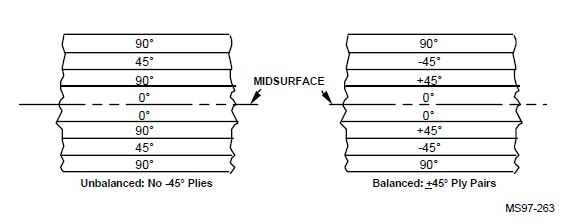
\includegraphics[scale=1.0]{figura/BalancedLaminate}
	\legend{Fonte: \cite{mil2002handbook}}
\end{figure}

Portanto, satisfazendo esta prática de projeto de utilizar somente laminados balanceados, tem-se a seguinte \autoref{eq_result_loadingA} resultante para tensão-deformação

\begin{equation} \label{eq_result_loadingA}
\begin{bmatrix}
    N_{x} \\
    N_{y} \\
    N_{xy} \\
\end{bmatrix}
=
\begin{bmatrix}
    A_{11} & A_{12} & 0\\
    A_{12} & A_{22} & 0\\
    0 & 0 & A_{66}\\
\end{bmatrix}
\begin{bmatrix}
    \varepsilon_{x}^o \\
    \varepsilon_{y}^o \\
    \gamma_{xy}^o \\
\end{bmatrix}
\end{equation}

\subsection{Regra dos 10\%}
Esta prática de projeto não é determinada por documentação  para ser rigorosamente seguida e também não há nenhuma documentação formal que comprove a sua validade. No entanto, esta prática foi seguida por diversas campanhas de projetos de estruturas em materiais compostos e demonstrou bons resultados e portanto, é adotada até os dias atuais em diversos programas. A regra dos 10\% determina que cada ângulo de laminação (0$^{\circ}$,$\pm$45$^{\circ}$ e 90$^{\circ}$) compreenda em pelo menos 10\% das camadas do laminado final. O uso desta prática de projeto conduz a laminados utilizáveis que são mais robustos pelo fato de que eles menos susceptíveis à fragilidade associada aos laminados rigorosamente ortotrópicos \cite{nasa1997guidelines}.

Além disso, segundo \cite{mil2002handbook}, um comportamento do laminado dominado pela matriz, ou seja, efeitos não lineares, pode ser evitados em laminados onde a direção principal da fibra não é alinhada com o eixo principal do carregamento.


% % ----------------------------------------------------------
% % Metodologia
% % ----------------------------------------------------------
%  \chapter[Metodologia]{Metodologia}

 \section{Desenvolvimento geral}
Visando realizar a otimização estrutural de um painel reforçado utilizando os parâmetros de laminação, realizou-se uma sequência de passos conformo segue:
\begin{enumerate}
  \item Análise teórica de um painel reforçado de material metálico utilizando a metodologia do \emph{Fator de Eficiência de Farrar} proposta por \cite{niu1997airframe}
  \item Otimização de um painel reforçado de material metálico utilizando o \emph{MSC Nastran} e comparação dos resultados obtidos com o resultado teórico obtido no item anterior. Nesta etapa visou-se obter a validação o método de otimização utilizado para assim poder aplicá-lo em outros paineis reforçados;
  \item Otimização de um painel reforçado de material composto utilizando o \emph{MSC Nastran} e comparação dos resultados obtidos com os resultados obtidos para um painel reforçado de material metálico.
\end {enumerate}

As seções seguintes descrevem a metodologia utilizada com mais detalhes e apresentam os modelos das otimizações realizadas e o capítulo seguinte contém os resultados obtidos.

\section{Análise teórica de um painel reforçado}
Visando realizar a análise teórica de um painel reforçado fabricado em material metálico, assume-se algumas proposições como segue e considera-se um painel conforme mostrado na \autoref{fig_StiffenedPanels}.

\begin{itemize}
\item Painel suficientemente largo para permitir que seja tratado como uma simples coluna, ou seja, não há restrições impostas nas bordas longitudinais do painel;
\item O painel possui uma fixação de apoio no final da sua estrutura, em relação ao comprimento L. Deve-se levar em consideração este comprimento como sendo o o comprimento efetivo do painel, e não o comprimento da báia;
\item As nervuras não colocam restrições à flambagem.
\end{itemize}

\begin{figure}[h]
	\caption{\label{fig_StiffenedPanels}Típico painel reforçado.}
  \centering
  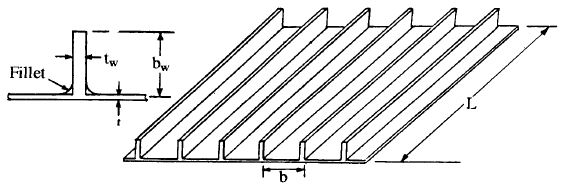
\includegraphics[scale=1.0]{figura/StiffenedPanel}
	\legend{Fonte: \cite{niu1997airframe}}
\end{figure}
\

Nota-se que\

$t$ -  Espessura do revestimento \

$b$ - Largura entre reforçadores \

$t_w$ - Espessura do reforçador \

$b_w$ - Altura do reforçador \

$L$ - Comprimento efetivo \
\

A \autoref{fig_InitialBuckling} mostra a tensão de flambagem inicial de diversas combinações de paineis reforçados, como razão entre $\dfrac{f_i}{f_o}$, considerando a seguinte notação.

\begin{figure}[h]
	\caption{\label{fig_InitialBuckling}Tensão inicial de flambagem.}
  \centering
  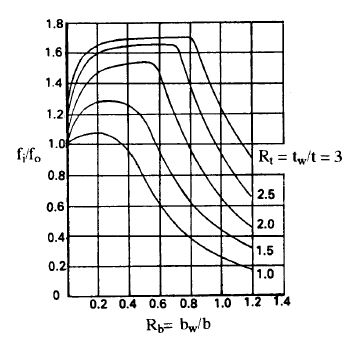
\includegraphics[scale=1.0]{figura/InitialBuckling}
	\legend{Fonte: \cite{niu1997airframe}}
\end{figure}
\
$f$ - Tensão aplicada\

$f_E$ - Tensão de instabilidade de Euler\

$f_i$ - Tensão inicial de flambagem do painel\

$f_o$ - Tensão inicial de flambagem de um painel reforçado longo, com espaçamento entre reforçadores (b) e espessura do revestimento (t), simplesmente apoiado ao longo da borda = 3.62$E_t$$(\dfrac{t}{b})^2$\

Segundo \cite{niu1997airframe}, para um dado material, no qual a relação entre $f$ e $E_t$ é conhecida, o \emph{Fator de Eficiência de Farrar} pode ser dado por:

\begin{equation} \label{Farrar}
F = f(\dfrac{L}{N E_t})^{0.5}
\end{equation}
Onde

$N$ - Carga por unidade de comprimento do painel (lbs/in)\

$E_t$ - Módulo tangente (psi)

\begin{figure}[h]
	\caption{\label{fig_plotFarrar}Tensão no painel \emph{vs.} índice estrutural $\dfrac{N}{L}$ para material Al 2024-T3.}
  \centering
  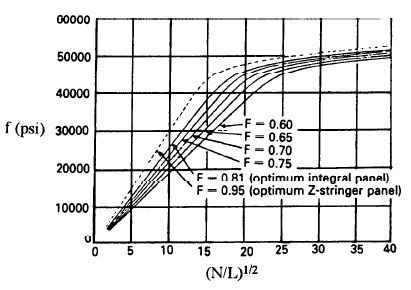
\includegraphics[scale=1.0]{figura/PlotFarrar}
	\legend{Fonte: \cite{niu1997airframe}}
\end{figure}
\

Este fator pode ser utilizado, conforme \autoref{fig_plotFarrar} que mostra para um painel reforçado de Al 2024-T3.

Sabe-se que a tensão incial de flambagem ($f_i$) é dada por:

\begin{equation} \label{InitialBuck}
f_i = (\dfrac{f_i}{f_o})[{3.62E_t(\dfrac{t}{b})^2}]
\end{equation}

E que a tensão de instabilidade de Euler ($f_E$) é dada por:

\begin{equation} \label{InitialEuler}
f_E = {\pi^2}E_t(\dfrac{\rho}{L})^2
\end{equation}

Onde $\rho$ corresponde ao raio de giração do painel reforçado em relação ao seu eixo neutro e tem que:

\begin{equation} \label{giracao}
{\rho^2} = {\dfrac{b^2{R_b}^3R_t}{12(1+R_bR_t)}}(4+R_bR_t)^2
\end{equation}

Em que
\begin{equation} \label{Rb}
R_b = \dfrac{b_w}{b}
\end{equation}
\

\begin{equation} \label{Rt}
R_t = \dfrac{t_w}{t}
\end{equation}

Relacionando a tensão no painel com a intensidade de carga tem-se:

\begin{equation} \label{StressPanel}
f = \dfrac{N}{t(1+R_bR_t)}
\end{equation}

Portanto, impõe-se a condição de que tensão aplicada é igual à tensão inicial de flambagem do painel que é igual à tensão de instabilidade de Euler ($f=f_i=f_E$).

Tomando-se a \autoref{InitialBuck} x \autoref{InitialEuler} x {\autoref{StressPanel}$^2$, obtem-se:

\begin{equation} \label{StressPanel2}
f^4 = \pi^2{E_t}^2(\frac{3.62{\rho}^2f_i}{f_ob^2L^2})[\dfrac{N^2}{(1+R_bR_t)^2}]
\end{equation}

Tirando a raiz quarta de ambos os lados, tem-se:

\begin{equation} \label{StressPanel3}
f = F(\dfrac{NE_t}{L})^{0.5}
\end{equation}

Onde o \emph{Fator de Eficiência de Farrar} vale:

\begin{equation} \label{Farrar_Efficiency}
F = 1.314{\dfrac{{R_b}^3R_t(4+R_bR_t)^{0.25}}{(1+R_bR_t)}}({\frac{f_i}{f_o}})^{0.25}
\end{equation}

\subsection{Limitação de projeto - Espaçamento entre reforçadores}
Considerando um espaçamento entre reforçadores (b) já previamente determinado, devido ao modelo em elementos finitos que foi desenvolvido para as etapas de otimização, tem-se, portanto, uma limitação de projeto. Segundo \cite{niu1997airframe}, para manter o valor de largura entre reforçadores constante (b) e o valor de espessura do reforçador também constante ($t_w$), tem-se as seguintes equações, que também são plotadas na \autoref{fig_plotstiffener}.

No caso deste estudo, considerou-se somente que a largura entre os reforçadores será constante, visando obter os outros parâmetros geométricos do painel reforçado ótimo.

\begin{figure}[ht]
	\caption{\label{fig_plotstiffener}Curvas para projetos com limitações - Espessura do reforçador ($t_w$) e largura do reforçador (b).}
  \centering
  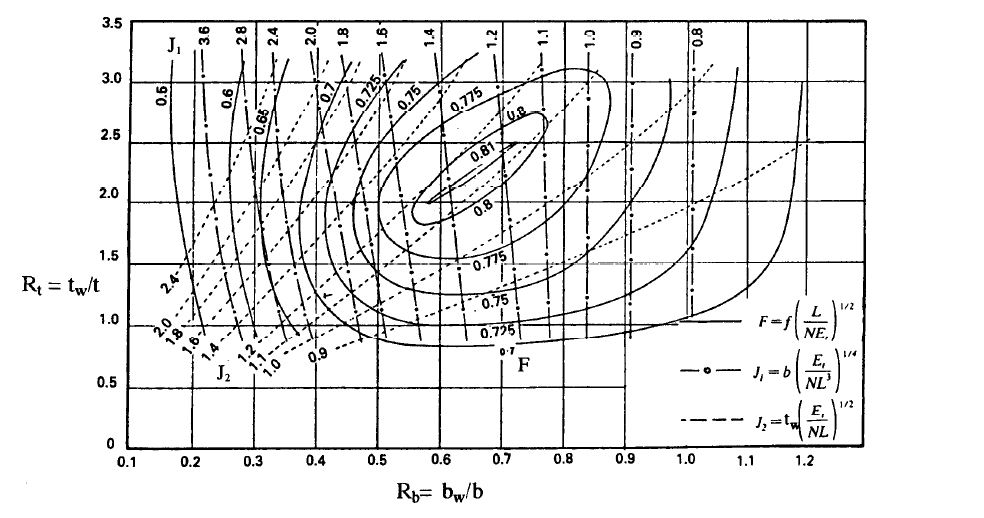
\includegraphics[scale=1.0]{figura/PlotStiffener}
	\legend{Fonte: \cite{niu1997airframe}}
\end{figure}
\

Visando, portanto, projetar um painel reforçado otimizado, seguindo a metodologia de \emph{Fator de Eficiência de Farrar} proposta por \cite{niu1997airframe}, submetido a uma carga de intensidade N, alguns passos foram seguidos.

\begin{itemize}
\item Utilização de valores otimizados \

F=0.81; $R_t$=2.25; $R_b$=0.65z\

\end{itemize}

\section{Otimização de um painel reforçado em material metálico}
Realizou-se uma otimização de um painel reforçado em material metálico utilizando o \emph{MSC Nastran}, para que após a validação do otimizador ele possa ser aplicado para outros tipos de paineis reforçados, como os em material composto.

\subsection{Modelo em elementos finitos}
Desenvolveu-se um modelo em elementos finitos de um painel reforçado, conforme \autoref{fig_StiffMetal} para realizar a análise de otimização. Este modelo foi desenvolvido utilizando somente um tipo de material, tanto para o revestimento quanto para o reforçador, que foi o Al, com as características conforme mostrado na %\autoref{fig_matmetal}.

\begin{figure}[ht]
	\caption{\label{fig_StiffMetal}Modelo do reforçador em material metálico.}
  \centering
  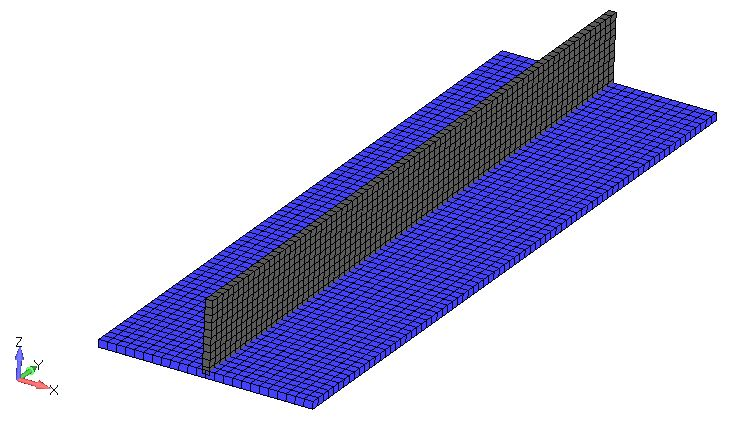
\includegraphics[scale=0.7]{figura/StiffMetal}
	\legend{Fonte: Femap}
\end{figure}
\

O modelo foi desenvolvido com elementos do tipo placa (\emph{PLATE}) para o reforçador e para o revestimento, e com duas propriedades distintas, sendo uma propriedade para o revestimento e outra propriedade para o reforçador.

O painel reforçado foi modelado utilizando somente a idealização de um reforçador e para isso as seguintes condições de contorno foram aplicadas, conforme mostrado na (adicionar figura). %\autoref{fig_StiffMetalConst}.

Em relação ao carregamento do aplicado no modelo, definiu-se que o painel reforçado estaria submetido somente a uma carga de compressão, sem cisalhamento. E portanto, aplicou-se essa carga de compressão conforme mostrado na \autoref{fig_StiffMetalLoad},
utilizando um elemento rígido do tipo RBE2 para distribuir a carga igualmente nos nós dos elementos de placa que situam-se em uma extremidade do reforçador.

\begin{figure}[h]
	\caption{\label{fig_StiffMetalLoad}Carregamento aplicado no reforçador em material metálico.}
  \centering
  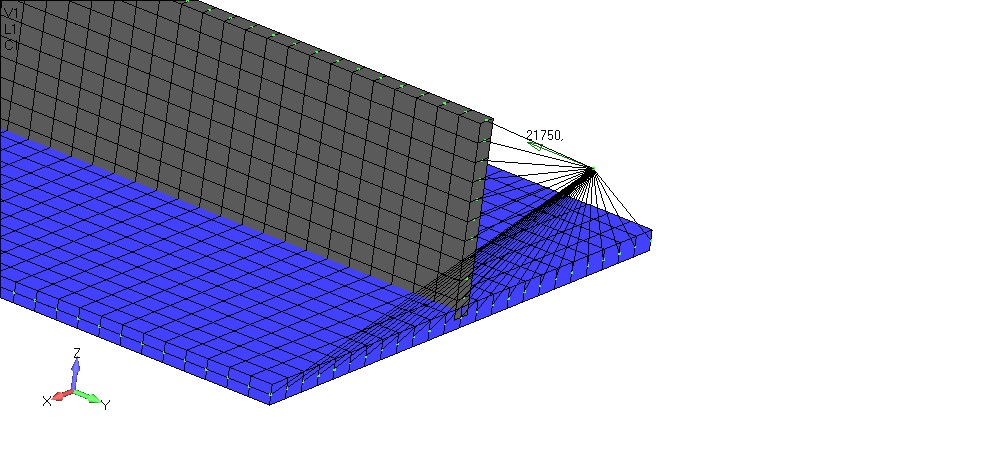
\includegraphics[scale=0.7]{figura/StiffMetalLoad}
	\legend{Fonte: Femap}
\end{figure}
\

\subsection{Otimização}
Em relaçao a otimização, buscou-se como objetivo minimizar o peso da estrutura. Portanto, durante a solução de otimização, mateve-se a carga de compressão constante e variou-se as espessuras do revestimento e do reforçador. Buscou-se, então, uma estrutura que suportasse a carga de compressão, utilizando uma análise de flambagem dentro do otimizador (SOL 105), e que possuíse o menor peso estrutural.

Resumidamente, a otimização possuiu as seguintes características:
\begin{itemize}
\item Função objetivo: minimizar o peso da estrutura;
\item Variáveis de projeto: espessura do revestimento e espessura do reforçador;
\item Respostas de projeto: Cinco (5) primeiros autovalores da solução de flambagem;
\item Restrições de projeto: Autovalores maiores que um (1);
\item Soluções utilizadas: Otimização (SOL 200) e Análise de flambagem (SOL 105).
\end{itemize}

\section{Otimização de um painel reforçado em material composto}
Após a realização da otimização do painel reforçado em material metálico, realizou-se a otimização de um painel reforçado em material composto utilizando o \emph{MSC Nastran}.

\subsection{Modelo em elementos finitos}
Similarmente ao modelo para o painel reforçado em material metálico, desenvolveu-se um modelo em elementos finitos de um painel reforçado em material composto, conforme \autoref{fig_StiffComposite} para realizar a análise de otimização.

\begin{figure}[ht]
 \caption{\label{fig_StiffComposite}Modelo do reforçador em material composto.}
 \centering
 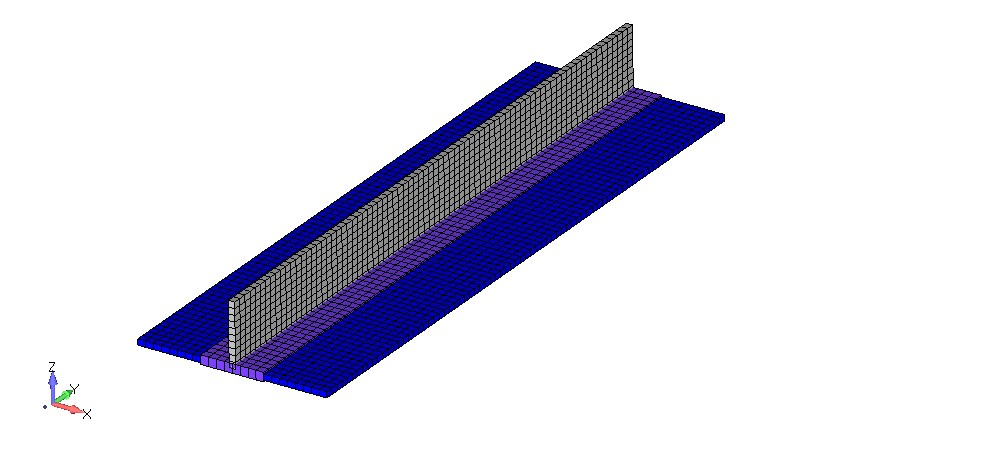
\includegraphics[scale=0.7]{figura/StiffComposite}
 \legend{Fonte: Femap}
\end{figure}
\

Este modelo foi desenvolvido utilizando como material composto o carbono, mas com duas propriedades de materiais distintas. Sendo que tem-se um material exclusivamente para o revestimento e outro para a alma do reforçador. Já a base do reforçador é composta tanto pelo material do revestimento, quanto pelo material da alma do reforçador, conforme ilustrado na \autoref{fig_StiffCompositeMaterial}.

\begin{figure}[ht]
 \caption{\label{fig_StiffCompositeMaterial}Visualização do reforçador em material composto.}
 \centering
 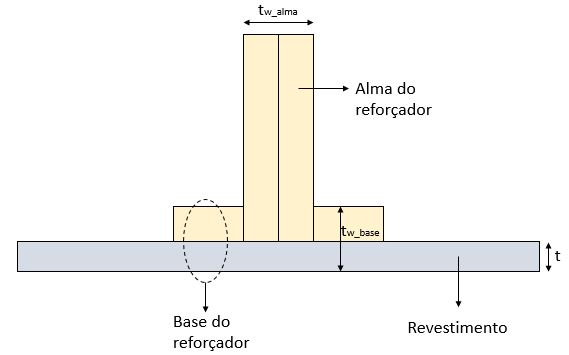
\includegraphics[scale=0.7]{figura/StiffCompositeMaterial}
 \legend{Fonte: Femap}
\end{figure}
\

O modelo foi desenvolvido com elementos do tipo placa (\emph{PLATE}) para o reforçador e para o revestimento, e com duas propriedades distintas, sendo uma propriedade para o revestimento e outra propriedade para o reforçador. Portanto, tem-se uma dada espessura para o reforçador ($t_{w alma}$), uma espessura para o revestimento (t) e uma espessura para a base do reforçador ($t_{w base}$) que é uma relação entre a espessura da alma do reforçador e a espessura do revestimento.

Optou-se por modelar a base do refoçador de material composto visando fazer a conexão entre as propriedades dos materiais da alma do reforçador e do revestimento.

O painel reforçado foi modelado utilizando somente a idealização de um reforçador, as condições de contorno aplicadas no modelo de elementos finitos de reforçador em material composto são as mesmas que foram aplicadas no modelo do reforçador em material metálico, conforme mostrado na (adicionar figura). %\autoref{fig_StiffMetalConst}.

Em relação ao carregamento do aplicado no modelo, definiu-se que o painel reforçado estaria submetido somente a uma carga de compressão, sem cisalhamento. E portanto, aplicou-se essa carga de compressão igualmente àquela aplicada no modelo do reforçador de material metálico, conforme mostrado na \autoref{fig_StiffMetalLoad}. Utilizou-se um elemento rígido do tipo RBE2 para distribuir a carga igualmente nos nós dos elementos de placa que situam-se em uma extremidade do reforçador.

\subsection{Otimização}
Em relaçao a otimização, buscou-se como objetivo minimizar o peso da estrutura. Portanto, durante a solução de otimização, mateve-se a carga de compressão constante e variou-se as espessuras do revestimento e do reforçador. Buscou-se, então, uma estrutura que suportasse a carga de compressão, utilizando uma análise de flambagem dentro do otimizador (SOL 105), e que possuíse o menor peso estrutural.

Resumidamente, a otimização possuiu as seguintes características:
\begin{itemize}
\item Função objetivo: minimizar o peso da estrutura;
\item Variáveis de projeto: espessura do revestimento e espessura do reforçador;
\item Respostas de projeto: Cinco (5) primeiros autovalores da solução de flambagem;
\item Restrições de projeto: Autovalores maiores que um (1);
\item Soluções utilizadas: Otimização (SOL 200) e Análise de flambagem (SOL 105).
\end{itemize}

%
% % ----------------------------------------------------------
% % Resultados
% % ----------------------------------------------------------
% \chapter[Resultados]{Resultados}

\section{Análise teórica vs. Otimização do painel reforçado}
Esta seção está dividida em três subseções:
\begin{itemize}
\item Resultados da análise teórica do painel reforçado;
\item Resultados da otimização do painel reforçado fabricado em material metálico;
\item Comparação dos dois itens ateriores .
\end{itemize}

\subsection{Análise teórica do painel reforçado}
A análise teórica do painel reforçado seguiu a metodologia do \emph{Fator de Eficiência de Farrar} proposta por \cite{niu1997airframe}. O painel reforçado foi submetido a uma carga de compressão de intensidade 10000daN (22480lbs), obtendo-se portando uma carga de compressão linear (N) como segue:\\~\\

\centerline{N = 833,3 N/mm = 4758,5 lbs/in}\


Utilizou-se os valores otimizados na análise teórica:
F=0.81; $R_t$=2.25; $R_b$=0.65;
Da \autoref{fig_plotFarrar}, encontrou-se o valor de "f" correspondente a carga por largura (4758,5 lbs/in), utilizando F=0.81 para o Al 2024-T3 extrudado.\\~\\


\centerline{f = 41000 psi}\

Encontrou-se o módulo tangente $E_t$ correspondente ao valor de "f", da curva de módulo tangente do material, conforme \autoref{fig_tangentmodulus}.\\~\\

\centerline{$E_t$ = 5.0x$10^6$ psi}
\

Conforme \autoref{Farrar_Efficiency_t} e \autoref{Farrar_Efficiency_tw}, determinou-se os valores de $t$ e $t_w$.\\~\\

\centerline{$t = 0.501({\dfrac{NL}{E_t}})^{0.5} = 0.06 in = 1.53 mm$}\

\centerline{$t_w = 2.25t = 0.136in = 3.46 mm$}\


\subsection{Otimização do painel reforçado em material metálico}

\subsection{Comparação dos resultados}

\section{Análise teórica vs. Otimização do painel reforçado}
Esta seção está dividida em três subseções:
\begin{itemize}
\item Resultados da otimização do painel reforçado fabricado em material metálico;
\item Resultados da otimização do painel reforçado fabricado em material composto;
\item Comparação dos dois itens ateriores .
\end{itemize}

\subsection{Otimização do painel reforçado em material metálico}

\subsection{Otimização do painel reforçado em material composto}

\subsection{Comparação dos resultados}


% ----------------------------------------------------------
% Finaliza a parte no bookmark do PDF
% para que se inicie o bookmark na raiz
% e adiciona espaço de parte no Sumário
% ----------------------------------------------------------
\phantompart
%
% % ---
% % Conclusão
% % ---
% % \chapter{Conclusão}
%
% - a fazer -

% % ---

% ----------------------------------------------------------
% ELEMENTOS PÓS-TEXTUAIS
% ----------------------------------------------------------
\postextual
% ----------------------------------------------------------

% ----------------------------------------------------------
% Referências bibliográficas
% ----------------------------------------------------------
\bibliography{bibliografia}

% ----------------------------------------------------------
% Glossário
% ----------------------------------------------------------
%
% Consulte o manual da classe abntex2 para orientações sobre o glossário.
%
%\glossary
%
% % ----------------------------------------------------------
% % Apêndices
% % ----------------------------------------------------------
% % % ---
% % Inicia os apêndices
% % ---
% \begin{apendicesenv}
%
% % Imprime uma página indicando o início dos apêndices
% \partapendices
%
% \chapter{apendice1}
%
% \chapter{apendice2}
%
% \end{apendicesenv}

%
%
% % ----------------------------------------------------------
% % Anexos
% % ----------------------------------------------------------
% % % ---
% % Inicia os anexos
% % ---
% \begin{anexosenv}
%
% % Imprime uma página indicando o início dos anexos
% \partanexos
%
% \chapter{anexo1}
%
% \chapter{anexo2}
%
% \end{anexosenv}

%
% %---------------------------------------------------------------------
% % INDICE REMISSIVO
% %---------------------------------------------------------------------
% \phantompart
% \printindex
% %---------------------------------------------------------------------

\end{document}
